\documentclass[10pt]{article}
\usepackage{colm2026}
\usepackage{amsmath,amssymb}
\usepackage{booktabs}
\usepackage{graphicx}
\usepackage{float}

\title{Supplementary Material:\\
       Delphi-Psychometric Evaluation of 3D Generative Models}

\author{Suki Wang \\ Roblox \\ \texttt{siqiwang@roblox.com}}

\date{Stanford AIMS Workshop on AI Measurement Science @ COLM 2026}

\begin{document}
\maketitle

\section{Robustness Checks}
\label{app:robustness}

\paragraph{E5: Leave-one-model-out cross-validation.}
We validated the tinyEval3D 30-item subset by holding out each model in turn,
re-selecting items from the remaining five models using difficulty-stratified
sampling, and measuring ranking recovery across all six held-out models.
The difficulty-stratified strategy yields mean LOO-CV Spearman $\rho=0.954$,
indicating robust generalisation to unseen models.
The IRT-$\theta$-stratified strategy achieves the same LOO-CV $\rho=0.954$,
as prompt generatability scores are stable across this leave-one-out perturbation.
Both substantially outperform what Fisher-information maximisation achieved
under the old (unstable, $N=6$ persons) IRT orientation, confirming that the
flipped 2PL orientation is the key enabler.

\paragraph{E3, E4: Dichotomization threshold sensitivity.}
We re-ran E3 on geometric consistency with thresholds at 3, 4, 6, and 7
(out of 9), alongside the main threshold of 5.
The proportion of zero-variance items is \emph{not} monotonic in threshold:
it is U-shaped (threshold=3: 48.2\%, threshold=4: 31.2\%, threshold=5:
7.8\%, threshold=6: 9.4\%, threshold=7: 81.4\%), because a zero-variance
item is one where all six models agree (all pass or all fail), which is
common at extreme thresholds (almost everyone passes a very low bar, or
almost everyone fails a very high one) and rare in the middle. Threshold=5
is close to the minimum of this curve, which is additional support for it
as the main-text choice rather than an arbitrary midpoint. The
difficulty-stratified subset strategy is robust to threshold choice as long
as sufficient non-zero-variance items remain (threshold $\leq 6$
recommended, based on this curve).

\paragraph{E2: Judge sensitivity.}
The judge facet accounts for only 1.7\% of variance, and ICC values
(0.81--0.88 per criterion) confirm high inter-judge reliability.
Dropping any single judge shifts mean scores by less than 0.3 points on the
0--9 scale; model rankings are stable across all three leave-one-judge-out
conditions (Spearman $\rho\geq0.90$ relative to three-judge consensus).

\paragraph{E2: Modeling-choice robustness (fixed vs.\ random criterion; raw
vs.\ standardized scale).}
Table~\ref{tab:vc_robustness} compares three specifications of the E2
variance decomposition on the automated-score stream: (i) the main-text
model, with criterion as a fixed effect and model$\times$criterion,
prompt$\times$criterion interactions included; (ii) an alternative treating
criterion as a random facet (no criterion interactions, matching the simpler
model used in an earlier draft); and (iii) the random-facet specification
applied to per-criterion $z$-scored scores. All three agree that criterion
(or its scale) dominates on the raw score, and that standardizing removes
this by construction while reallocating variance mainly to prompt and model.
Table~\ref{tab:vc_robustness_delphi} shows the same three specifications for
the Delphi stream, where criterion's share is already small on the raw scale
(6--7\%) because judges rate all criteria on a common 0--9 scale, so
standardization changes the picture only modestly.

\begin{table}[H]
\centering
\small
\caption{Automated-score stream: \% of total variance under three
specifications. ``---'' marks a facet not present in that specification
(fixed-criterion interactions are undefined under a random-criterion model,
and vice versa). Column sums equal 100\% in each specification.}
\label{tab:vc_robustness}
\begin{tabular}{lrrr}
\toprule
Facet & Fixed criterion & Random criterion & Random criterion, $z$-scored \\
\midrule
Criterion                 & 82.0\% & 84.7\% & 0.0\% \\
Residual                  & 10.1\% & 11.4\% & 59.8\% \\
Model$\times$Criterion    &  2.1\% & --- & --- \\
Model$\times$Prompt       &  2.0\% &  1.2\% &  4.7\% \\
Prompt$\times$Criterion   &  1.5\% & --- & --- \\
Model                     &  1.4\% &  1.6\% & 14.8\% \\
Prompt                    &  0.9\% &  1.1\% & 20.7\% \\
\midrule
Total                     & 100.0\% & 100.0\% & 100.0\% \\
\bottomrule
\end{tabular}
\end{table}

\begin{table}[H]
\centering
\small
\caption{Delphi stream: \% of total variance under the same three
specifications.}
\label{tab:vc_robustness_delphi}
\begin{tabular}{lrrr}
\toprule
Facet & Fixed criterion & Random criterion & Random criterion, $z$-scored \\
\midrule
Model                     & 37.3\% & 37.4\% & 41.2\% \\
Residual                  & 16.9\% & 22.4\% & 22.1\% \\
Model$\times$Prompt       & 14.1\% & 13.6\% & 14.8\% \\
Prompt                    & 12.9\% & 13.9\% & 15.1\% \\
Criterion                 &  6.0\% &  6.6\% &  0.0\% \\
Prompt$\times$Criterion   &  5.4\% & --- & --- \\
Round                     &  4.5\% &  4.3\% &  4.7\% \\
Judge                     &  1.7\% &  1.8\% &  2.1\% \\
Model$\times$Criterion    &  1.3\% & --- & --- \\
\midrule
Total                     & 100.0\% & 100.0\% & 100.0\% \\
\bottomrule
\end{tabular}
\end{table}

Notably, prompt$\times$criterion is the fourth-largest facet in the Delphi
stream (5.4\%)---larger than criterion's own main effect and than
model$\times$criterion (1.3\%)---indicating that some prompts are
differentially easy or hard depending on which criterion a judge is applying.
This interaction was omitted from an earlier draft of the model with no
stated justification; it does not change which facet dominates (model
quality), but it is large enough that its exclusion should not be assumed
harmless without checking, as we do here.

\paragraph{E2: The automated scorer as a fourth rater.}
To directly compare rater severity across measurement instruments, we treat
the automated scorer as a fourth rater alongside the three Delphi judges,
restricted to the 100 prompts $\times$ 5 models both streams cover and to
judges' Round~1 (independent, pre-anchor) scores to avoid circularity with
the automated score already being shown to judges from Round~2 onward
(main text, Delphi protocol). Because the automated scorer's per-criterion
ranges differ sharply from the judges' uniform 0--9 scale (main text, E2), we
$z$-score each criterion across all four raters before comparing severity
or fitting any model---otherwise scale differences would masquerade as
severity differences.

\begin{table}[H]
\centering
\small
\caption{Rater severity (mean $z$-score; more negative = harsher) and
variance components with vs.\ without the automated scorer as a fourth
rater. Criterion treated as a fixed effect, as in the main text's Table~3.}
\label{tab:rater_severity}
\begin{tabular}{lrr}
\toprule
& 3 LLM judges only & + automated (4 raters) \\
\midrule
Gemini severity     & $-0.386$ & $-0.322$ \\
Automated severity   & --- & $-0.290$ \\
Claude severity      & $-0.100$ & $-0.011$ \\
GPT severity         & $+0.487$ & $+0.625$ \\
\midrule
Model (\% variance)  & 32.2\% & 23.6\% \\
Residual (\% variance) & 25.7\% & 42.3\% \\
Judge (\% variance)  & 17.4\% & 17.5\% \\
\bottomrule
\end{tabular}
\end{table}

The automated scorer's severity sits between Gemini and Claude---harsher
than Claude, comparable to Gemini---so it is not a severity outlier
relative to the LLM judges. Adding it leaves judge variance essentially
unchanged (17.4\%$\to$17.5\%), but residual variance rises sharply
(25.7\%$\to$42.3\%) while model variance falls correspondingly
(32.2\%$\to$23.6\%): the automated scorer's disagreement with the LLM
judges is not a fixed calibration offset (which would show up as judge
variance) but idiosyncratic, item-level disagreement (residual)---a harder
form of disagreement to correct for than a simple severity adjustment.

\paragraph{E1/E3: Pooled IRT across all four raters.}
We further pool all four raters' person-level ratings---(model, prompt,
rater) triples, not judge-averaged scores---into a single graded-response
IRT model (criteria as items, as in E1's MIRT), recoding each criterion
onto a common 5-category scale via quantile bins computed across the
pooled data so the differing native ranges do not distort item category
structure. Within this single fitted model, splitting $\hat\theta$ by
rater type reproduces the same split as the separate per-stream fits in
the main text: automated-only $\hat\theta$ ranks HunyuanDiT-3D highest
($-0.02$) and TRELLIS second ($-0.16$); Delphi-judge-only $\hat\theta$
ranks TRELLIS highest ($0.69$) and HunyuanDiT-3D second ($0.58$). The
pooled estimate (both rater types combined) narrowly favors TRELLIS
($0.475$ vs.\ HunyuanDiT-3D's $0.432$), but each model receives 100
automated person-rows against roughly 300 Delphi-judge person-rows (three
judges $\times$ 100 prompts), so the pooled estimate is not a neutral
adjudication between the two methods---it simply reflects that Delphi
contributes three times as many rated instances per model.

\subsection*{Delphi Protocol Flowchart}

\begin{figure}[H]
  \centering
  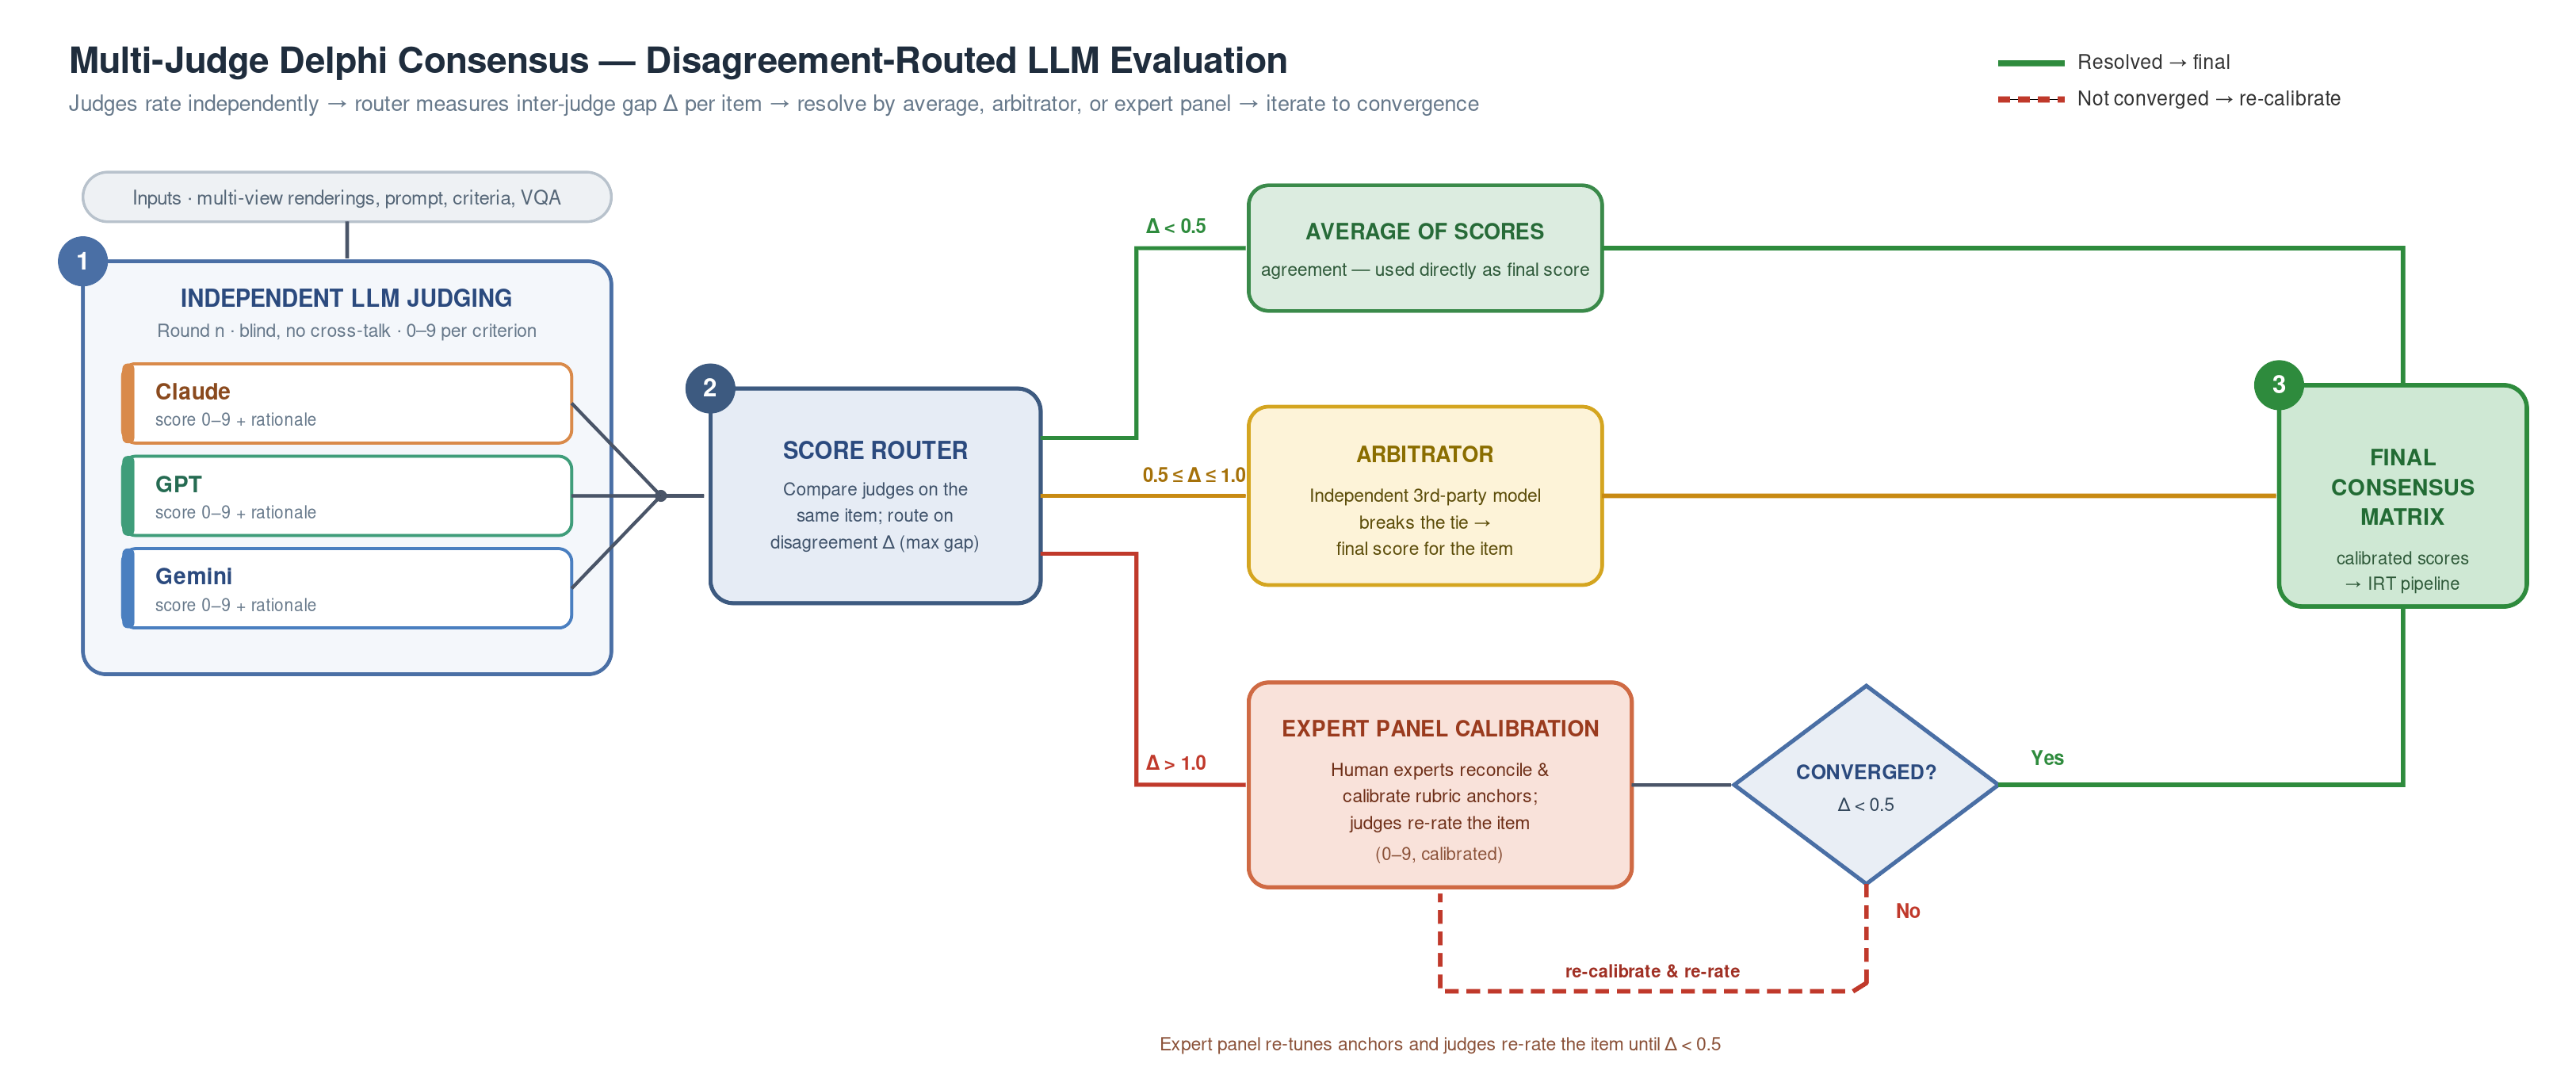
\includegraphics[width=0.95\linewidth]{delphi_process_flowchart.png}
  \caption{Delphi-structured LLM judging protocol. Three vision-capable LLM
    judges rate each (model, prompt) pair independently in Round~1, then
    receive anonymized group statistics and a dissent summary before
    re-rating in Rounds~2 and~3. Round~3 is skipped when inter-judge SD
    drops below 1.0 on $\geq4$ of 5 criteria after Round~2.}
  \label{fig:delphi_flowchart}
\end{figure}

\end{document}
